\section{Savage and Prescott Benchmark}
\label{sec:benchmarks:savageprescott}

This benchmark problem computes the viscoelastic (Maxwell) relaxation
of stresses from repeated infinite, strike-slip earthquakes in 3D
without gravity. The files needed to run the benchmark may be found
at \url{https://github.com/geodynamics/pylith_benchmarks/tree/master/quasistatic/sceccrustdeform/savageprescott}.
An analytical solution to this problem is described by Savage and
Prescott \cite{Savage:Prescott:1978}, which provides a simple way
to check our numerical solution. A python utility code is provided
in the utils directory to compute the analytical solution. Although
this problem is actually 2.5D (infinite along-strike), we solve it
using a 3D finite element model.


\subsection{Problem Description}

Figure \vref{fig:benchmark:savageprescott:geometry} shows the geometry
of the problem, as described by \cite{Savage:Prescott:1978}. The
analytical solution describes the surface deformation due to repeated
earthquakes on an infinite strike-slip fault embedded in an elastic
layer overlying a Maxwell viscoelastic half-space. The upper portion
of the fault (red in the figure) is locked between earthquakes, while
the lower portion (blue in the figure) creeps at plate velocity. At
regular recurrence intervals, the upper portion of the fault abruptly
slips by an amount equal to the plate velocity multiplied by the recurrence
interval, thus 'catching up' with the lower part of the fault.

There are some differences between the analytical solution and our
numerical representation. First, the analytical solution represents
the earthquake cycle as the superposition of uniform fault creep and
an elementary earthquake cycle. Uniform fault creep is simply the
uniform movement of the two plates past each other at plate velocity.
For the elementary earthquake cycle, no slip occurs below the locked
portion of the fault (blue portion in the figure). On the locked (red)
portion of the fault, backslip equal to plate velocity occurs until
the earthquake recurrence interval, at which point abrupt forward
slip occurs. In the finite element solution, we perform the simulation
as described in the figure. Velocity boundary conditions are applied
at the extreme edges of the model to simulate block motion, steady
creep is applied along the blue portion of the fault, and regular
earthquakes are applied along the upper portion of the fault. It takes
several earthquake cycles for the velocity boundary conditions to
approximate the steady flow due to steady block motion, so we would
not expect the analytical and numerical solutions to match until several
earthquakes have occurred. Another difference lies in the dimensions
of the domain. The analytical solution assumes an infinite strike-slip
fault in an elastic layer overlying a Maxwell viscoelastic half-space.
In our finite element model we are restricted to finite dimensions.
We therefore extend the outer boundaries far enough from the region
of interest to approximate boundaries at infinity.

Due to the difficulties in representing solutions in an infinite domain,
there are several meshes that have been tested for this problem. The
simplest meshes have uniform resolution (all cells have equal dimensions);
however, such meshes typically do not provide accurate solutions since
the resolution is too coarse in the region of interest. For that reason,
we also tested meshes where the mesh resolution decreases away from
the center. In the problem description that follows, we will focus
on the hexahedral mesh with finer discretization near the fault
({\tt meshes/hex8\_6.7km.exo.gz}), which provides a good match
with the analytical solution. It will first be necessary to gunzip
this mesh so that it may be used by PyLith.
\begin{description}
\item [Domain] The domain for this mesh spans the region
\begin{gather*}
-1000\leq x\leq1000\ km,\\
-500\leq y\leq500\ km,\\
-400\ km\leq z\leq0.
\end{gather*}
The top (elastic) layer occupies the region $-40\ km\ \leq z\leq0$
and the bottom (viscoelastic) layer occupies the region $-400\ km\ \leq z\leq-40\ km$.
\item [Material~properties] The material is a Poisson solid with a shear
modulus ($\mu$) of 30 GPa. The domain is modeled using an elastic
isotropic material for the top layer and a Maxwell viscoelastic material
for the bottom layer. The bottom layer has a viscosity ($\eta$) of
2.36682e+19 Pa-s, yielding a relaxation time ($2\eta/\mu$) of 50
years.
\item [Fault] The fault is a vertical, left-lateral strike-slip fault.
The strike is parallel to the y-direction at the center of the model:
\begin{gather*}
x=0\ km,\\
-500\leq y\leq500\ km,\\
-40\ km\leq z\leq0.
\end{gather*}
The locked portion of the fault (red section in Figure \vref{fig:benchmark:savageprescott:geometry})
extends from $-20\: km\leq z\leq0$, while the creeping section (blue)
extends from $-40\: km\leq z\leq0$. Along the line where the two
sections coincide ($z=-20\: km$), half of the coseismic displacement
and half of the steady creep is applied (see \texttt{finalslip.spatialdb}
and \texttt{creeprate.spatialdb}).
\item [Boundary~conditions] On the bottom boundary, vertical displacements
are set to zero, while on the y-boundaries the x-displacements are
set to zero. On the x-boundaries, the x-displacements are set to zero,
while constant velocities of +/- 1 cm/yr are applied in the y-direction,
giving a relative plate motion of 2 cm/year.
\item [Discretization] For the nonuniform hexahedral mesh, the resolution
at the outer boundaries is 20 km. An inner region is then put through
one level of refinement, so that near the center of the mesh the resolution
is 6.7 km. All meshes were generated with CUBIT.
\item [Basis~functions] We use trilinear hexahedral cells.
\item [Solution] We compute the surface displacements and compare these
to the analytical solution in Figure \vref{fig:benchmark:savageprescott:solution}.
\end{description}

\begin{figure}[htbp]
  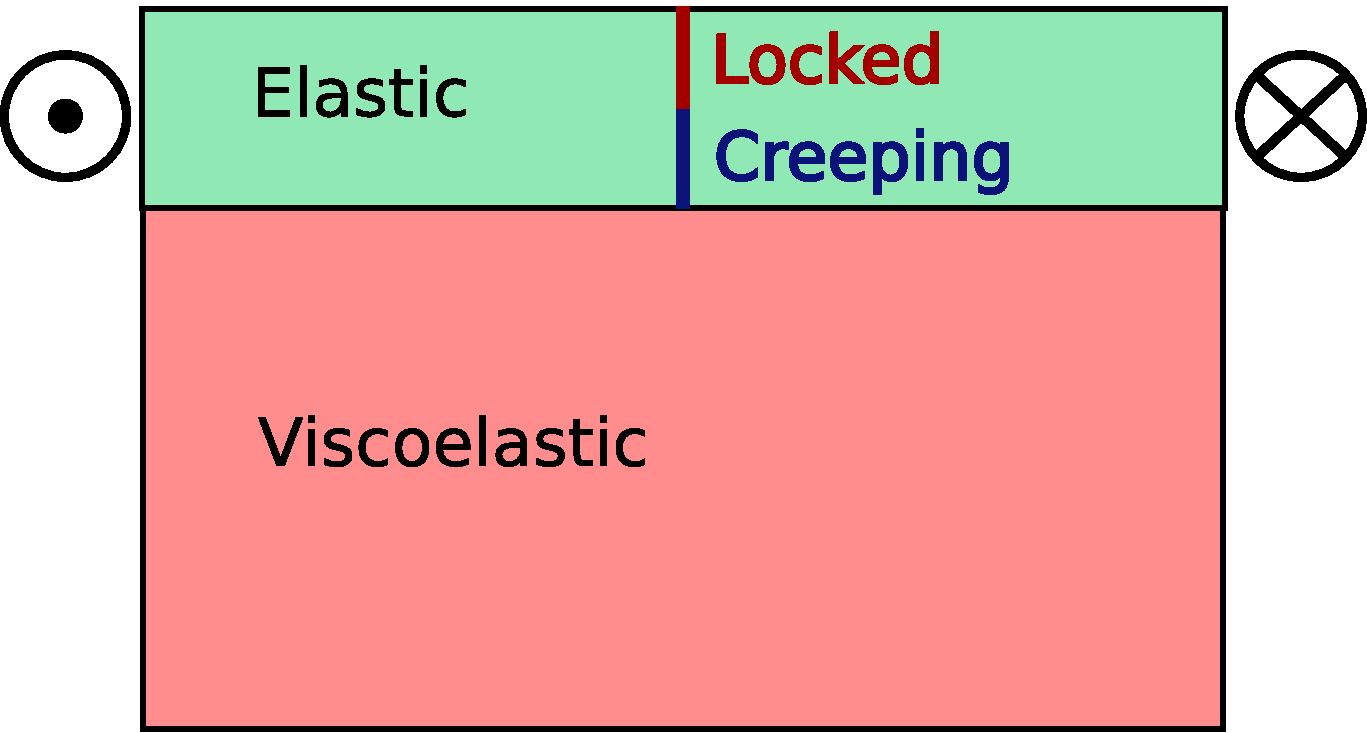
\includegraphics[scale=0.33]{benchmarks/figs/savageprescott_diagram}
  \caption{Problem description for the Savage and Prescott strike-slip
    benchmark problem.}
  \label{fig:benchmark:savageprescott:geometry}
\end{figure}


\subsection{Running the Benchmark}

There are a number of {\tt .cfg} files corresponding to the
different meshes, as well as a {\tt pylithapp.cfg} file defining
parameters common to all problems. Each problem uses four
{\tt .cfg} files: {\tt pylithapp.cfg}, {\tt fieldsplit.cfg}
(algrebraic multigrid preconditioner), a cell-specific file (e.g.,
{\tt hex8.cfg}), and a resolution specific file (e.g.,
hex8\_6.7km.cfg).

\begin{shell}
# If you have not do so already, checkout the benchmarks from the CIG Git repository.
$ git clone https://github.com/geodynamics/pylith_benchmarks.git
# Change to the quasistatic/sceccrustdeform/savageprescott directory.
$ cd quasistatic/sceccrustdeform/savageprescott
# Decompress the gzipped files in the meshes directory.
$ gunzip meshes/*.gz
# Run one of the simulations.
$ pylith hex8.cfg hex8_6.7km.cfg fieldsplit.cfg
\end{shell}

Each simulation uses 10 earthquake cycles of 200 years each,
using a time-step size of 10 years, for a total simulation time of
2000 years. Ground surface output occurs every 10 years, while all
other outputs occur every 50 years.

Once the problem has run, results will be placed in the {\tt output}
directory. These results may be viewed directly using 3-D
visualization software such as ParaView; however, to compare results
to the analytical solution, some postprocessing is required. First,
generate the analytical results by running the {\tt calc\_analytic.py}
script. This will produce files with displacements and velocities
({\tt analytic\_disp.txt} and {\tt analytic\_vel.txt}) in the {\tt
  output} directory that are easy to use with a plotting package, such
as matplotlib or Matlab.


\subsection{Benchmark Results}

Figure \vref{fig:benchmark:savageprescott:solution} shows the computed
surface displacements for the 10th earthquake cycle compared with
the analytical solution. The profile results were obtained as described
above, and then all results (analytical and numerical) were referenced
to the displacements immediately following the last earthquake. We
find very good agreement between the analytical and numerical solutions,
even for meshes with uniform refinement. We have not yet explored
quantitative fits as a function of mesh resolution. For this benchmark,
it is also important to consider the distance of the boundary from
the region of interest. Also note that the agreement between analytical
and numerical solutions is poor for early earthquake cycles, due to
the differences in simulating the problem, as noted above.

\begin{figure}[htbp]
  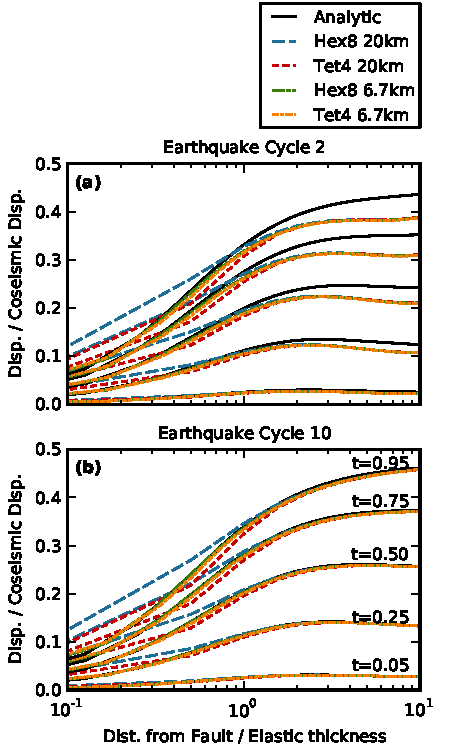
\includegraphics[scale=0.66]{benchmarks/figs/savageprescott_soln_profiles}
  \caption{Displacement profiles perpendicular to the fault for a
    PyLith simulation with hex8 cells and the analytical solution for
    earthquake cycle 10.}
  \label{fig:benchmark:savageprescott:solution}
\end{figure}

% End of file
